\section{Usability Principles}
Much progress has been made in the design of application, such that users enjoy using a site and are therefore more likely to recommend it and to reuse the site. David Benyon composed usability principles which act as a guideline when designing applications with the users in mind \cite{Benyon}. These principles aim to improve consistency, familiarity and intuitiveness of applications.

The screenshots in figure \ref{fig:Twitter_Changes} highlight how the design of websites have changed. In particular, the design in image \ref{fig:Twitter_2017} shows how Twitter now use a more simplistic flat design, which uses bright colours so key areas of the page a clearly visible and separated. This is as opposed to the design in \ref{fig:Twitter_2006}, which uses a lot of gradients. This draws attention away from the important features in the site and makes it appear more cluttered. This shows how the designs have been adapted in order to make them more usable. Fidelis will also aim to make the application more usable through the use of design principles, as discussed in this section.

\begin{figure}[H]
	\centering
	\begin{subfigure}[t]{0.45\textwidth}
		\centering
		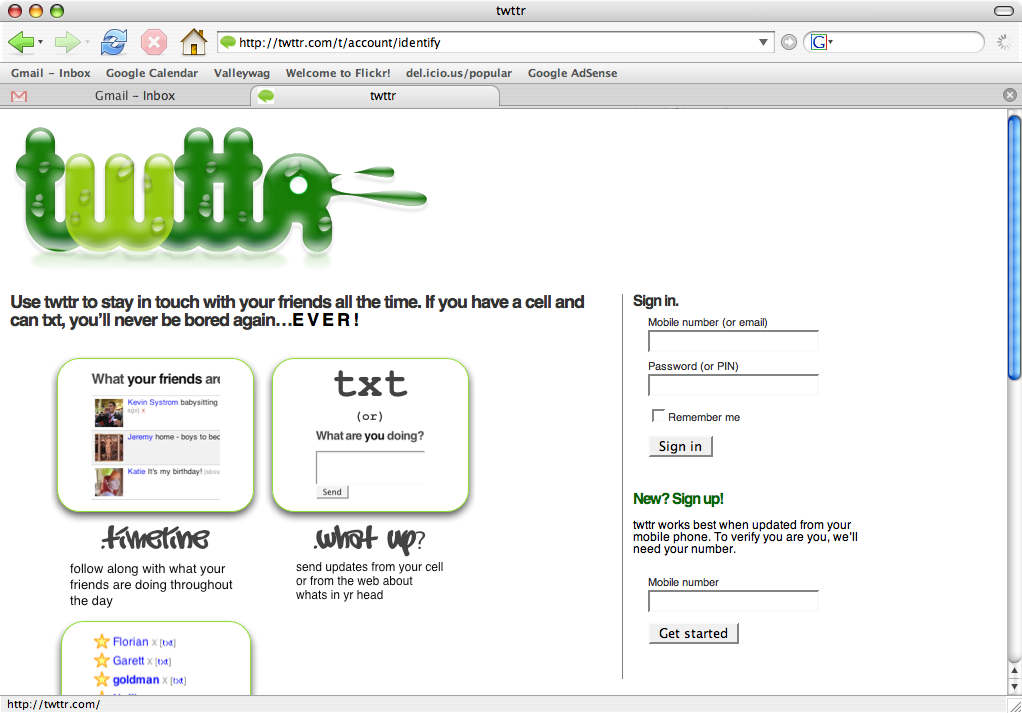
\includegraphics[width=1.0\textwidth, height=125px]{Images/Design/Twitter_2006}
		\caption{Twitter in 2006}\label{fig:Twitter_2006}		
	\end{subfigure}
	\quad
	\begin{subfigure}[t]{0.45\textwidth}
		\centering
		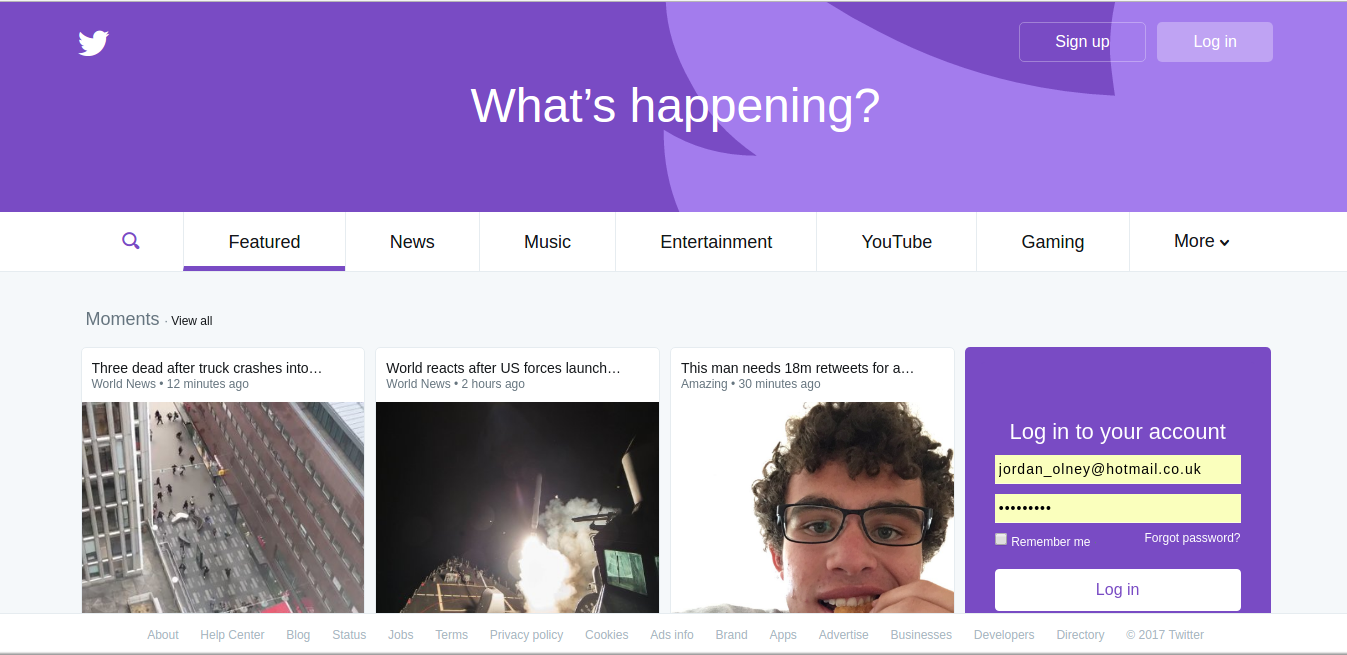
\includegraphics[width=1.0\textwidth, height=125px]{Images/Design/Twitter_2017}
		\caption{Twitter in 2017}\label{fig:Twitter_2017}
	\end{subfigure}
	\caption{Twitter in 2006 and 2017}\label{fig:Twitter_Changes}
\end{figure}

\subsection{Consistency}
By ensuring that the design of the application is consistent across all pages in the site, users will be able to learn quickly about how to use the features of the site and how to navigate more easily. An example of this is the navigation bar, which will be used in all of the pages, allowing the user to search and log in and out. Figure \ref{fig:navs} demonstrates how Facebook and Twitter have designed a similar navigation bar which features throughout their site. In addition, Fidelis will make use of widgets, which can then be reproduced across the site. This allows features to be reproduced, without the style having to change, allowing the users to understand the possible actions they are able to make on each page and improving ease of use.

\subsection{Familiarity}
Whilst aiming to differentiate Fidelis from other social networks by implementing features which make it more trust-centric, keeping a familiar design will allow users to use the site with minimum learning. Therefore, the language being used in the site will be similar to the language in pre-existing social networks. This includes the terms `following' and `followers' to describe who a user is connected to within the network and `trending' to show the most common terms which are being mentioned within a period of time. In addition, the hash symbol will be used to tag a post and @ will be use to mention a user in a post, as is the case with social networks such as Twitter, Instagram and Facebook. Other features such as profile picture, wallpapers and notifications will also follow a familiar format in comparison with current popular websites.

\subsection{Intuitive Design}